 \section{Using TMVA}
\label{sec:usingtmva}

A typical TMVA classification or regression analysis consists of two independent phases: 
the {\em training} phase, where the multivariate methods are trained, tested and 
evaluated, and an {\em application} phase, where the chosen methods are applied to 
the concrete classification or regression problem they have been trained for.
An overview of the code flow for these two phases as implemented in the 
examples \code{TMVAClassification.C}\index{TMVAClassification} and 
\code{TMVAClassificationApplication.C}\index{TMVAClassificationApplication} 
(for classification -- see Sec.~\ref{sec:examplejob}), and 
\code{TMVARegression.C}\index{TMVARegression} and 
\code{TMVARegressionApplication.C}\index{TMVARegressionApplication} (for regression)
are sketched in Fig.~\ref{fig:TMVAflow}. Multiclass classification does not differ much from
two class classification from a technical point of view and differences will only be highlighted
where neccessary.
 
In the training phase, the communication of the user with the data sets and the 
MVA methods is performed via a \code{Factory} object, created at the beginning of 
the program. The TMVA Factory provides member functions to specify the training 
and test data sets, to register the discriminating input and -- in case of 
regression -- target variables, and to 
book the multivariate methods. Subsequently the Factory calls for 
training, testing and the evaluation of the booked MVA methods. Specific 
result (``weight'') files are created after the training phase by each booked 
MVA method.

The application of training results to a data set with unknown sample composition 
(classification) / target value (regression) is governed by the \code{Reader} object. 
During initialisation, the user registers the input variables\footnote
{
  This somewhat redundant operation is required to verify the correspondence between
  the Reader analysis and the weight files used.
} 
together with their local memory addresses, and books the MVA methods that were found 
to be the most appropriate after evaluating the training results. As booking argument, the 
name of the weight file is given. The weight file provides for each of the methods full 
and consistent configuration according to the training setup and results. Within the 
event loop, the input variables are updated for each event and the MVA response
values are computed. Some methods also provide the computation of errors. 

For standalone use of the trained MVA methods, TMVA also generates lightweight 
C++ response classes, which contain the encoded information from the weight files
so that these are not required anymore (\cf\  Sec.~\ref{sec:usingtmva:standaloneClasses}).
\begin{figure}[p]
\begin{center}
   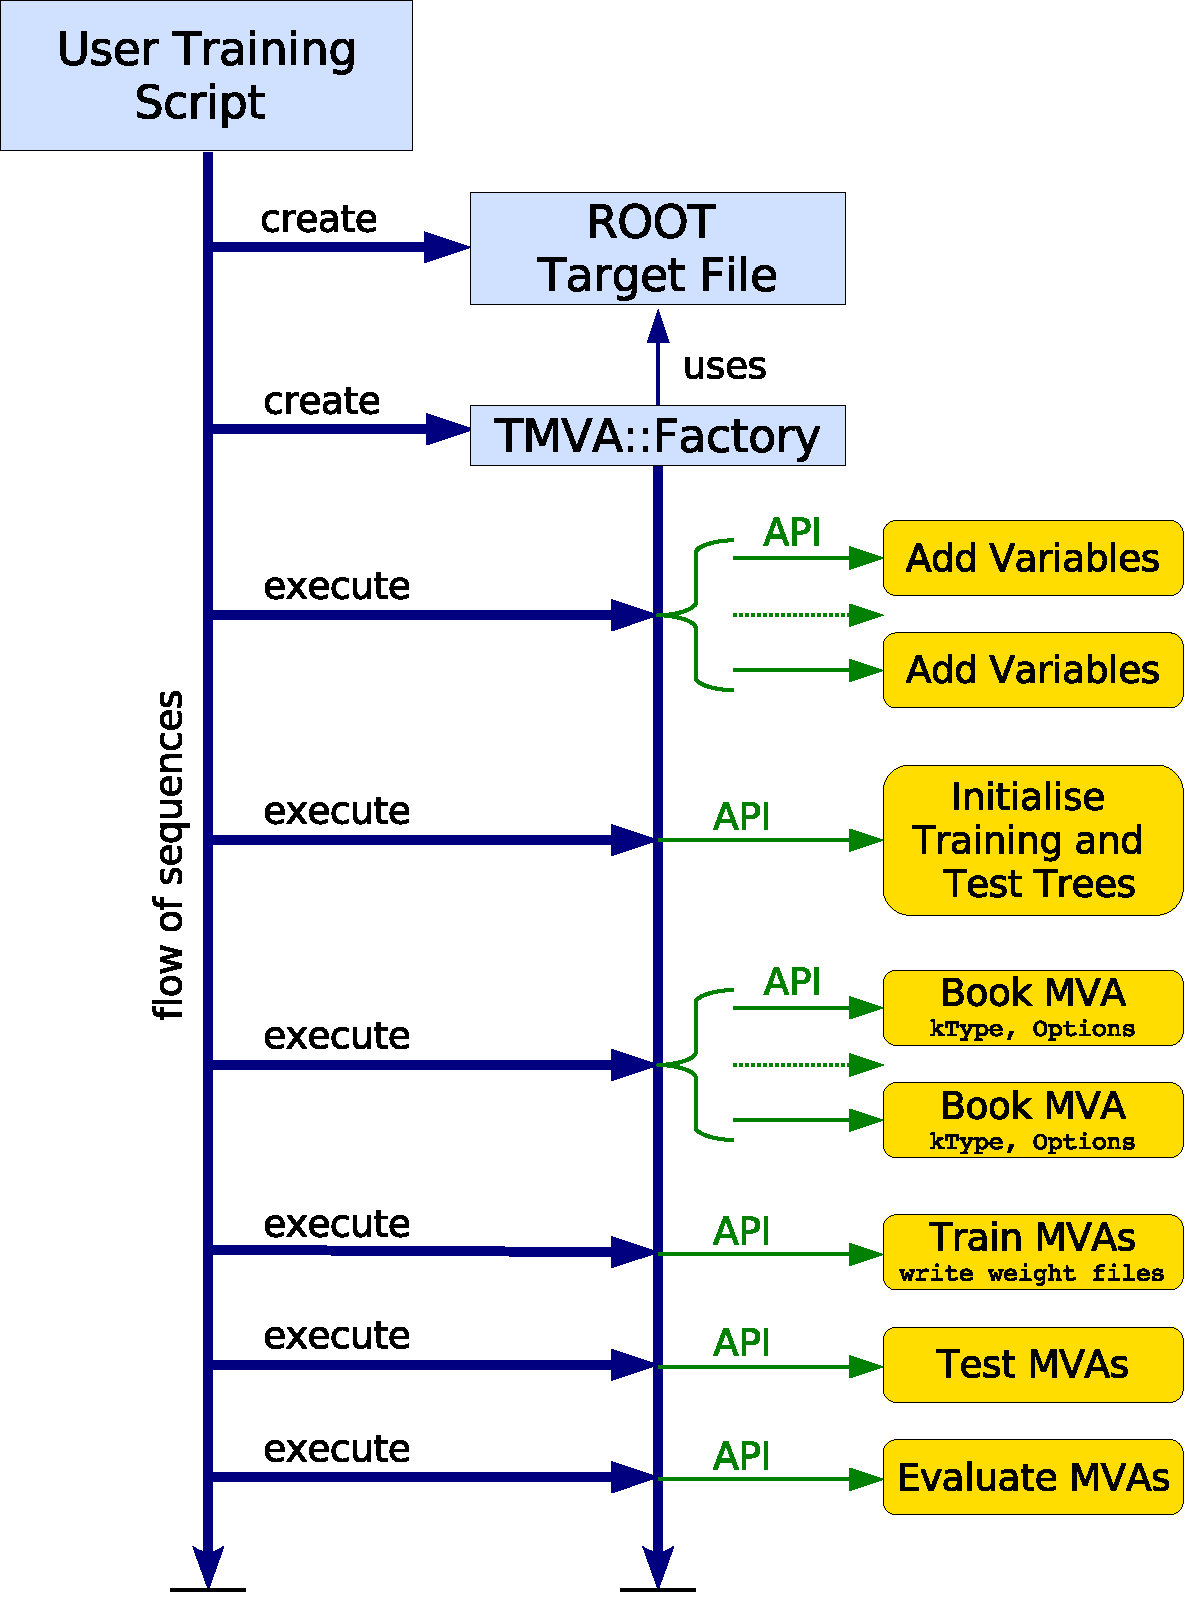
\includegraphics[width=0.50\textwidth]{plots/TMVAnalysisFlow}
   \hspace{-0.65cm}
   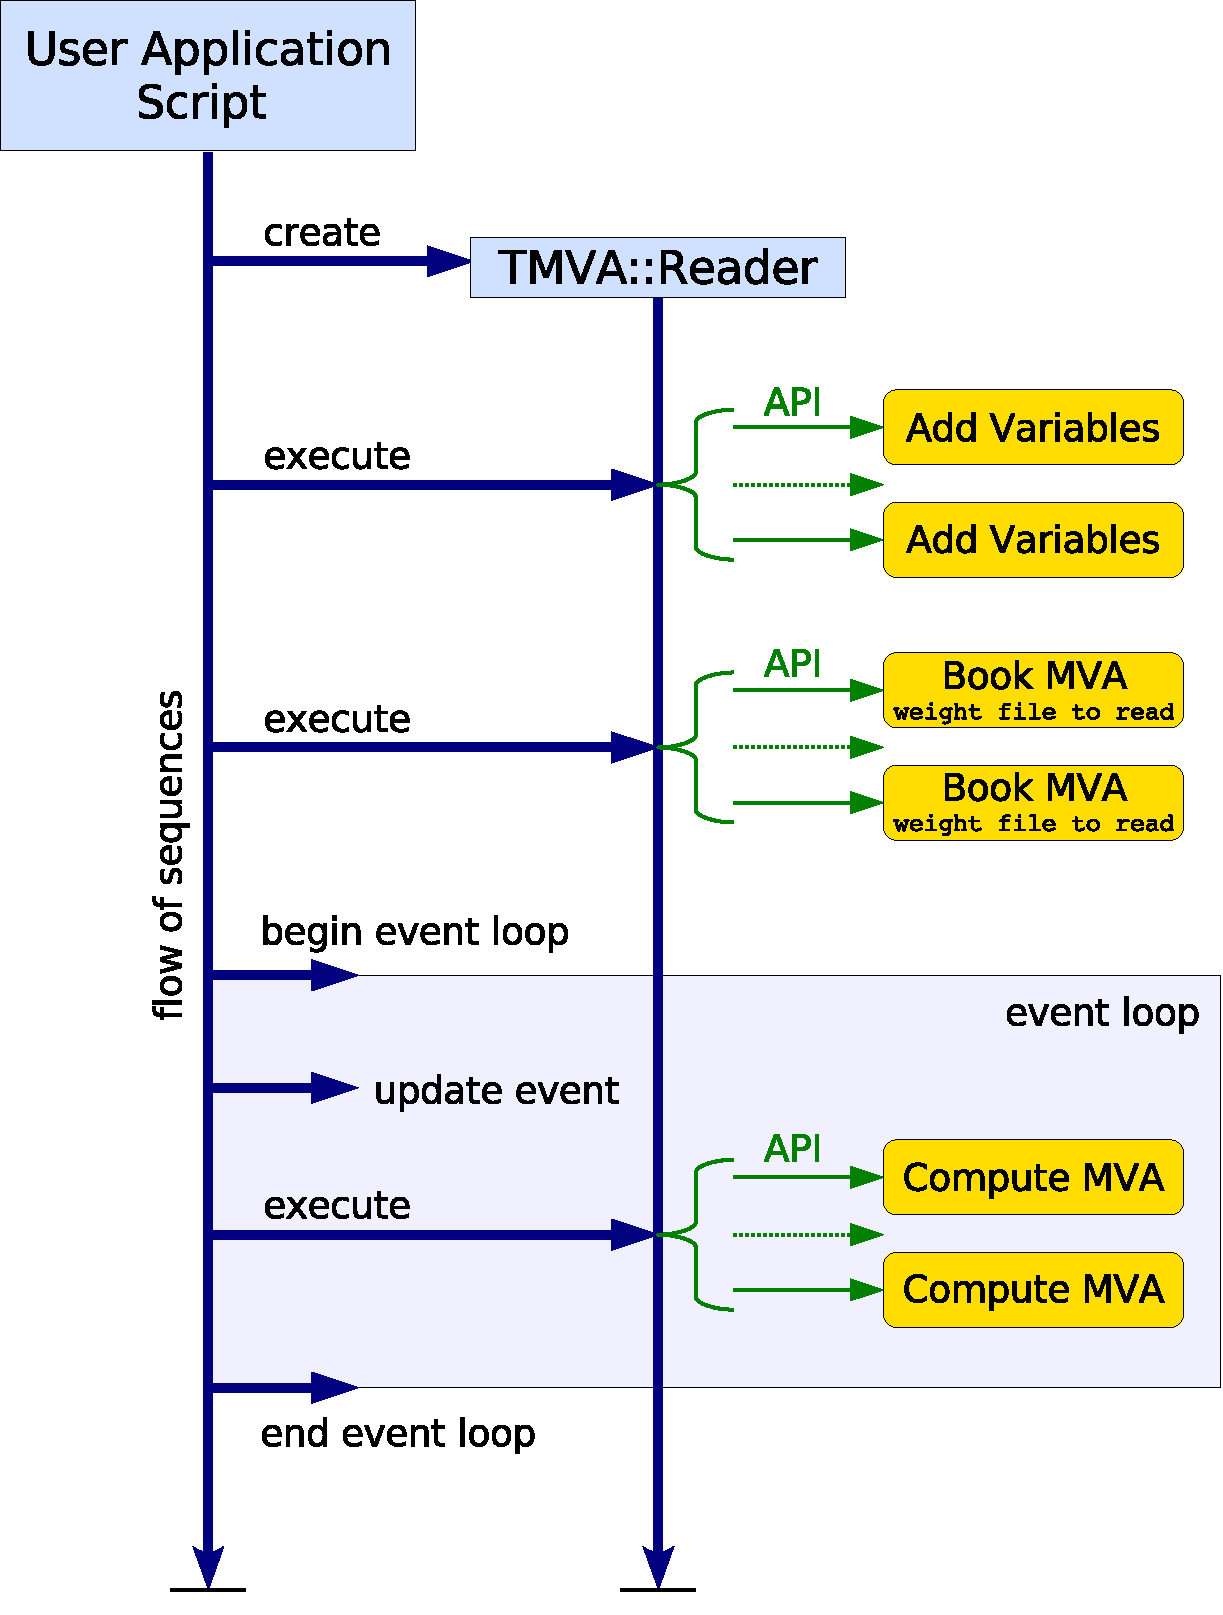
\includegraphics[width=0.516\textwidth]{plots/TMVAppFlow}
\end{center}
\vspace{-0.5cm}
\caption[.]{\underline{Left:} Flow (top to bottom) of a typical TMVA 
         training application.
         The user script can be a ROOT macro, C++ executable, python
         script or similar. The user creates a ROOT \code{TFile}, 
         which is used by the TMVA Factory to store output histograms 
         and trees. After creation by the user, the Factory organises the 
         user's interaction with the TMVA modules. It is the only TMVA object 
         directly created and owned by the user. First the discriminating
         variables that must be \code{TFormula}-compliant functions of 
         branches in the training trees are registered. For regression also
         the target variable must be specified. Then, selected MVA methods
         are booked through a type identifier and a user-defined unique name,
         and configuration options are specified via an option string. 
         The TMVA analysis proceeds by consecutively calling the training, 
         testing and performance evaluation methods of the Factory. The training 
         results for all booked methods are written to custom weight files in 
         XML format and the evaluation histograms are stored in the output file. 
         They can be analysed with specific macros that come with TMVA (\cf\  
         Tables~\ref{pgr:scripttable1} and \ref{pgr:scripttable2}). \\
         \underline{Right:} Flow (top to bottom) of a typical 
         TMVA analysis application. The MVA methods qualified by the preceding 
         training and evaluation step are now used to classify data of unknown 
         signal and background composition or to predict a regression target. 
         First, a \code{Reader} class object is created, which 
         serves as interface to the method's response, just as was the Factory 
         for the training and performance evaluation. The discriminating variables 
         and references to locally declared memory placeholders are registered
         with the Reader. The variable names and types must be equal to those
         used for the training. The selected MVA methods are booked with their 
         weight files in the argument, which fully configures them. The user 
         then runs the event loop, where for each event the values of the input
         variables are copied to the reserved memory addresses, and the MVA
         response values (and in some cases errors) are computed.
         \index{Factory}\index{Reader}\index{TMVA analysis flow}
}
\label{fig:TMVAflow}
\end{figure}

\subsection{The TMVA Factory\index{Factory}}

The TMVA training phase begins by instantiating a \code{Factory} object
with configuration options listed in Option-Table~\ref{opt:factory}.
\begin{codeexample}
\begin{tmvacode}
TMVA::Factory* factory 
           = new TMVA::Factory( "<JobName>", outputFile, "<options>" );
\end{tmvacode}
\caption[.]{\codeexampleCaptionSize Instantiating a Factory class object. The first 
            argument is the user-defined job name that will reappear in the names of 
            the weight files containing the training results. The second argument is the
            pointer to a writable \code{TFile} output file created by the user, where 
            control and performance histograms are stored. }
\end{codeexample}

% ======= input option table ==========================================
\begin{option}[t]
\input optiontables/Factory.tex
\caption[.]{\optionCaptionSize 
     Configuration options reference for class: {\em Factory}.  
     Coloured output is switched on by default, except when running ROOT in batch
     mode (\ie, when the '\code{-b}' option of the CINT interpreter is invoked). 
     The list of transformations contains a default set of data preprocessing steps 
     for test and visualisation purposes only. The usage of preprocessing transformations
     in conjunction with MVA methods must be configured when booking the methods.
}
\label{opt:factory}
\end{option}
% =====================================================================

\subsubsection{Specifying training and test data\index{Factory!specifying input data (trees)}}

The input data sets used for training and testing of the multivariate methods
need to be handed to the Factory. TMVA supports ROOT \code{TTree} and derived 
\code{TChain} objects as well as text files. If ROOT trees are used for classification
problems, the signal and background events can be located in the same or in different 
trees. Data trees can be provided specifically for the purpose of either training or testing or for both purposes. In the latter case the factory then splits the tree into one part for training, the other for testing (see also section \ref{sec:PreparingTrainingTestData}).

Overall weights can be specified for the signal and background training data 
(the treatment of event-by-event weights is discussed below).

Specifying {\bf classification training and test data} in ROOT tree format with signal 
and background events being located in different trees:
\begin{codeexample}
\begin{tmvacode}
// Get the signal and background trees from TFile source(s); 
// multiple trees can be registered with the Factory
TTree* sigTree  = (TTree*)sigSrc->Get( "<YourSignalTreeName>"   );
TTree* bkgTreeA = (TTree*)bkgSrc->Get( "<YourBackgrTreeName_A>" );
TTree* bkgTreeB = (TTree*)bkgSrc->Get( "<YourBackgrTreeName_B>" );
TTree* bkgTreeC = (TTree*)bkgSrc->Get( "<YourBackgrTreeName_C>" );

// Set the event weights per tree (these weights are applied in 
// addition to individual event weights that can be specified)
Double_t sigWeight  = 1.0; 
Double_t bkgWeightA = 1.0, bkgWeightB = 0.5, bkgWeightC = 2.0;

// Register the trees
factory->AddSignalTree    ( sigTree,  sigWeight  );
factory->AddBackgroundTree( bkgTreeA, bkgWeightA );
factory->AddBackgroundTree( bkgTreeB, bkgWeightB );
factory->AddBackgroundTree( bkgTreeC, bkgWeightC );
\end{tmvacode}
\caption[.]{\codeexampleCaptionSize Registration of signal and background ROOT trees
            read from \code{TFile} sources. Overall signal and background weights
            per tree can also be specified.
            The \code{TTree} object may be replaced by a \code{TChain}. The trees will be later split by the factory into subsamples used for testing and training.  }
\end{codeexample}

Specifying {\bf classification training and test data} in ROOT tree format with signal 
and background events being located in the same tree:
\begin{codeexample}
\begin{tmvacode}
TTree* inputTree = (TTree*)source->Get( "<YourTreeName>" );

TCut signalCut = ...;  // how to identify signal events 
TCut backgrCut = ...;  // how to identify background events

factory->SetInputTrees( inputTree, signalCut, backgrCut );
\end{tmvacode}
\caption[.]{\codeexampleCaptionSize Registration of a single ROOT tree containing the 
            input data for signal {\em and} background, read from a \code{TFile} source. 
            The \code{TTree} object may be replaced by a \code{TChain}. The cuts
            identify the event species.}
\end{codeexample}

Specifying {\bf classification data} in ROOT tree format with signal 
and background training/test events being located in separate trees:
\begin{codeexample}
\begin{tmvacode}
#include "TMVA/Types.h"
// Get the signal and background training and test trees from TFile source(s); 
TTree* sigTreeTrain = (TTree*)sigSrc->Get( "<YourSignalTrainTreeName>"   );
TTree* bkgTreeTrain = (TTree*)bkgSrc->Get( "<YourBackgrTrainTreeName>" );
TTree* sigTreeTest  = (TTree*)sigSrc->Get( "<YourSignalTestTreeName>" );
TTree* bkgTreeTest  = (TTree*)bkgSrc->Get( "<YourBackgrTestTreeName>" );

// Set the event weights (these weights are applied in 
// addition to individual event weights that can be specified)
Double_t sigWeight  = 1.0; 
Double_t bkgWeight = 1.0;

// Register the trees
factory->AddSignalTree    ( sigTreeTrain, sigWeight, TMVA::Types::kTraining);
factory->AddBackgroundTree( bkgTreeTrain, bkgWeight, TMVA::Types::kTraining);
factory->AddSignalTree    ( sigTreeTest,  sigWeight, TMVA::Types::kTesting);
factory->AddBackgroundTree( bkgTreeTest,  bkgWeight, TMVA::Types::kTesting);
\end{tmvacode}
\caption[.]{\codeexampleCaptionSize Registration of signal and background ROOT trees
            read from \code{TFile} sources.
            The first two tree are specified to be used only for training the other two only for testing. Please note that the tree type testing/training requires the inclusion of the header file TMVA/Types.h.}
\end{codeexample}

Specifying {\bf classification training and test data} in text format:
\begin{codeexample}
\begin{tmvacode}
// Text file format (available types: 'F' and 'I')
//   var1/F:var2/F:var3/F:var4/F
//   0.21293  -0.49200  -0.58425  -0.70591
//   ...
TString sigFile = "signal.txt";     // text file for signal
TString bkgFile = "background.txt"; // text file for background

Double_t sigWeight = 1.0; // overall weight for all signal events
Double_t bkgWeight = 1.0; // overall weight for all background events

factory->SetInputTrees( sigFile, bkgFile, sigWeight, bkgWeight );
\end{tmvacode}
\caption[.]{\codeexampleCaptionSize Registration of signal and background text files used for training and testing. 
            Names and types of the input variables are given in the first line, 
            followed by the values.}
\end{codeexample}
\clearpage
Specifying {\bf regression training and test data} in ROOT tree format:
\begin{codeexample}
\begin{tmvacode}
factory->AddRegressionTree( regTree, weight );  
\end{tmvacode}
\caption[.]{\codeexampleCaptionSize Registration of a ROOT tree containing the 
            input and target variables. An overall weight per tree can also be specified.
            The \code{TTree} object may be replaced by a \code{TChain}.
}
\end{codeexample}

Rather than having only global weighting factors for individual input
trees which allow to scale them to the same ``luminosity'', individual
event weights can be applied as well. These weights should be
available event-by-event, i.e. as a column or a function of columns of
the input data sets. To specify the weights to be used for the
training use the command:\index{Factory!specifying event weights}
\begin{codeexample}
\begin{tmvacode}
factory->SetWeightExpression( "<YourWeightExpression>" );
\end{tmvacode}

or if you have different expressions (variables) used as weights in the signal and background
trees:

\begin{tmvacode}
factory->SetSignalWeightExpression( "<YourSignalWeightExpression>" );
factory->SetBackgroundWeightExpression( "<YourBackgroundWeightExpression>" );
\end{tmvacode}
\caption[.]{\codeexampleCaptionSize Specification of individual weights for the 
            training events. The expression must be a function of variables present in 
            the input data set.}
\end{codeexample}

\subsubsection{Negative event weights\index{Negative Event Weights}}
\label{sec:NegativeEventWeights}

In next-to-leading order Monte Carlo generators, events with
(unphysical) negative weights may occur in some phase space
regions. Such events are often troublesome to deal with, and it
depends on the concrete implementation of the MVA method, whether or
not they are treated properly. Among those methods that correctly
incorporate events with negative weights are likelihood 
and multi-dimensional probability density estimators, but also 
decision trees. A summary of this feature for all TMVA methods is given in
Table~\ref{tab:methodStatus}. In cases where a method does {\em not}
properly treat events with negative weights, it is advisable to ignore
such events for the training - but to include them in the performance
evaluation to not bias the results. This can be explicitly requested for 
each MVA method via the boolean configuration option \code{IgnoreNegWeightsInTraining} 
(\cf\  Option Table~\ref{opt:mva::methodbase} on
page~\pageref{opt:mva::methodbase}). 


\subsubsection{Defining input variables, spectators and targets\index{Factory!selecting input variables}}
\label{sec:defineVariables}

The variables in the input trees used to train the MVA methods are registered 
with the Factory using the \code{AddVariable} method. It takes the variable name 
(string), which must have a correspondence in the input ROOT tree or input text file,
and optionally a number type (\code{'F'} (default) and \code{'I'}). The type is used 
to inform the method whether a variable takes continuous floating point or discrete 
values.\footnote
{
  For example for the projective likelihood method, a histogram out of discrete 
  values would not (and should not) be interpolated between bins. 
}
Note that \code{'F'} indicates {\em any} floating point type, \ie, \code{float} 
{\em and} \code{double}. Correspondingly, \code{'I'} stands for integer, 
{\em including} \code{int}, \code{short}, \code{char}, and the corresponding 
\code{unsigned} types. Hence, if a variable in the input tree is \code{double}, 
it should be declared \code{'F'} in the  \code{AddVariable} call. 

It is possible to specify variable expressions, just as for the \code{TTree::Draw} 
command (the expression is interpreted as a \code{TTreeFormula}, including the use 
of arrays). Expressions may be abbreviated for more concise screen output (and plotting) 
purposes by defining shorthand-notation {\em labels} via the assignment operator \code{:=}. 

In addition, two more arguments may be inserted into the \code{AddVariable} 
call, allowing the user to specify {\em titles} and {\em units} for the input variables 
for displaying purposes.

The following code example revises all possible options to declare an input variable:
\begin{codeexample}
\begin{tmvacode}
factory->AddVariable( "<YourDescreteVar>",                  'I' );
factory->AddVariable( "log(<YourFloatingVar>)",             'F' );
factory->AddVariable( "SumLabel := <YourVar1>+<YourVar2>",  'F' );
factory->AddVariable( "<YourVar3>", "Pretty Title", "Unit", 'F' );
\end{tmvacode}
\caption[.]{\codeexampleCaptionSize Declaration of variables used to train the
            MVA methods. Each variable is specified by its name in the training 
            tree (or text file), and optionally a type (\code{'F'} for 
            floating point and \code{'I'} for integer, \code{'F'} is default if 
            nothing is given). Note that \code{'F'} indicates {\em any} floating point
            type, \ie, \code{float} {\em and} \code{double}. Correspondingly, \code{'I'}
            stands for integer, {\em including} \code{int}, \code{short}, \code{char},
            and the corresponding \code{unsigned} types. Hence, even if a variable in 
            the input tree is \code{double}, it should be declared \code{'F'} here.             
            Here, \code{YourVar1} has discrete values and is thus declared 
            as an integer. Just as in the \code{TTree::Draw} command, it 
            is also possible to specify expressions of variables. The \code{:=} operator
            defines labels (third row), used for shorthand notation in screen outputs
            and plots. It is also possible to define titles and units for the variables
            (fourth row), which are used for plotting. If labels {\em and} titles are 
            defined, labels are used for abbreviated screen outputs, and titles for plotting. 
}
\label{ce:addvariable}
\end{codeexample}
It is possible to define {\em spectator variables}\index{Spectator variables}, which are 
part of the input data set, but which are not used in the MVA training, test nor during 
the evaluation. They are copied into the \code{TestTree}, together with the used input 
variables and the MVA response values for each event, where the spectator variables can 
be used for correlation tests or others. Spectator variables are declared as follows:
\begin{codeexample}
\begin{tmvacode}
factory->AddSpectator( "<YourSpectatorVariable>" );
factory->AddSpectator( "log(<YourSpectatorVariable>)" );
factory->AddSpectator( "<YourSpectatorVariable>", "Pretty Title", "Unit" );
\end{tmvacode}
\caption[.]{\codeexampleCaptionSize Various ways to declare a spectator variable, not 
            participating in the MVA anlaysis, but written into the final \code{TestTree}.
}
\end{codeexample}
For a regression problem, the target variable is defined similarly, without however 
specifying a number type:
\begin{codeexample}
\begin{tmvacode}
factory->AddTarget( "<YourRegressionTarget1>" );
factory->AddTarget( "log(<YourRegressionTarget2>)" );
factory->AddTarget( "<YourRegressionTarget3>", "Pretty Title", "Unit" );
\end{tmvacode}
\caption[.]{\codeexampleCaptionSize Various ways to declare the target variables used 
            to train a multivariate regression method. If the MVA method supports 
            multi-target (multidimensional) 
            regression\index{Regression!multi-target (multidimensional)}, 
            more than one regression target can be defined. 
}
\end{codeexample}

\subsubsection{Preparing the training and test 
               data\index{Factory!preparing training and test data}}
\label{sec:PreparingTrainingTestData}

The input events that are handed to the Factory are internally copied
and split into one {\em training} and one {\em test} ROOT tree. This
guarantees a statistically independent evaluation of the MVA
algorithms based on the test sample.\footnote { A fully unbiased
  training and evaluation requires at least three statistically
  independent data sets. See comments in Footnote~\ref{ftn:training}
  on page~\pageref{ftn:training}.  } The numbers of events used in
both samples are specified by the user. They must not exceed the
entries of the input data sets. In case the user has provided a ROOT
tree, the event copy can (and should) be accelerated by disabling all
branches not used by the input variables.

It is possible to apply selection requirements (cuts) upon the input
events. These requirements can depend on any variable present in the
input data sets, \ie, they are not restricted to the variables used by
the methods. The full command is as follows:
\begin{codeexample}
\begin{tmvacode}
TCut preselectionCut = "<YourSelectionString>";
factory->PrepareTrainingAndTestTree( preselectionCut, "<options>" );
\end{tmvacode}
\caption[.]{\codeexampleCaptionSize Preparation of the internal TMVA
  training and test trees. The sizes (number of events) of these trees
  are specified in the configuration option string. For classification
  problems, they can be set individually for signal and
  background. Note that the preselection cuts are applied before the
  training and test samples are created, \ie, the tree sizes apply to
  numbers of {\em selected} events. It is also possible to choose
  among different methods to select the events entering the training
  and test trees from the source trees. All options are described in
  Option-Table~\ref{opt:datasetfactory}. See also the text for further
  information.}
\label{ce:treePreparation}
\end{codeexample}
For {\bf classification}, the numbers of signal and background events
used for training and testing are specified in the configuration
string by the variables \code{nTrain_Signal},
\code{nTrain_Background}, \code{nTest_Signal} and
\code{nTest_Background} (for example,
\code{"nTrain_Signal=5000:nTrain_Background=5000:nTest_Signal=4000:nTest_Background=5000"}).
The default value (zero) signifies that all available events are
taken, \eg, if \code{nTrain_Signal=5000} and \code{nTest_Signal=0},
and if the total signal sample has 15000 events, then 5000 signal
events are used for training and the remaining 10000 events are used
for testing. If \code{nTrain_Signal=0} and \code{nTest_Signal=0}, the
signal sample is split in half for training and testing.  The same
rules apply to background. Since zero is default, not specifying
anything corresponds to splitting the samples in two halves.

For {\bf regression}, only the sizes of the train and test samples are given, \eg,
\code{"nTrain_Regression=0:nTest_Regression=0"}, so that one half of the input 
sample is used for training and the other half for testing. If a tree is 
given to the factory as a training tree. The events of that tree can only be used for training. The same is true for test trees. 

The option \code{SplitMode} defines how the training and test samples
are selected from the source trees. With \code{SplitMode=Random},
events are selected randomly. With \code{SplitMode=Alternate}, events
are chosen in alternating turns for the training and test samples as
they occur in the source trees until the desired numbers of training
and test events are selected. The training and test samples should 
contain the same number of events for each event class.
In the \code{SplitMode=Block} mode the
first \code{nTrain_Signal} and \code{nTrain_Background}
(classification), or \code{nTrain_Regression} events (regression) of
the input data set are selected for the training sample, and the next
\code{nTest_Signal} and \code{nTest_Background} or
\code{nTest_Regression} events comprise the test data. This is usually
not desired for data that contains varying conditions over the range
of the data set. For the \code{Random} selection mode, the seed of the
random generator can be set. With \code{SplitSeed=0} the generator
returns a different random number series every time.  The default seed
of 100 ensures that the same training and test samples are used each time 
TMVA is
run (as does any other seed apart from 0). The option \code{MixMode}
defines the order of how the training and test events of the different classes
are combined into a training sample. It also defines the order in which they appear in the test sample. The available options for
\code{MixMode} are the same as for \code{SplitMode}. By default, the same
option is chosen for the \code{MixMode} as given in \code{SplitMode}. Again, 
with \code{MixMode=Random}, the order of the events in the samples is random.
With \code{MixMode=Alternate} subsequent events are always of the next class
(e.g. 0, 1, 2, 3, 0, 1, 2, 3, $\cdots$). With \code{MixMode=Block} all events
of one class are inserted in a block into the training/test samples (e.g. 
0, 0, $\cdots$, 0, 1, 1, $\cdots$, 1, 2, 2, $\cdots$, 2, $\cdots$ ).

In some cases event weights are given by Monte Carlo generators, and
may turn out to be overall very small or large numbers. To avoid
artifacts due to this, TMVA can internally renormalise the signal and
background training(!) weights such that their respective sums of
effective (weighted) events is equal. This is the default
renormalisation and it can be modified with the configuration option
\code{NormMode} (\cf\ Table~\ref{opt:datasetfactory}).  Possible
settings are: \code{None}: no renormalisation is applied (the weights
are used as given), \code{NumEvents} : renormalisation of the training
events such that the sum of event weights of the Signal and Background
events, respectively are equal to the number of events \code{Ns, Nb}
requested in the call
\code{Factory::PrepareTrainingAndTestTree("","nTrain_Signal=Ns,nTrain_Background=Nb..."},
\code{EqualNumEvents} (default): the event weights are renormalised such
that both, the sum of all weighted signal training events equals the
sum of all weights of the background training events. Note: All this renormalisation only
affects the training events as the training of some classifiers is sensitive to the
relative amount of signal and background in the training data. On the other hand, the 
background or signal efficiency of the trained classifier as determined from the test
sample is independent of the relative abundance of signal and background events.

% ======= input option table ==========================================
\begin{option}[p]
\input optiontables/DataSetFactory.tex
\caption[.]{\optionCaptionSize Configuration options reference in call
  \code{Factory::PrepareTrainingAndTestTree(..)}.  For regression,
  \code{nTrain_Signal} and \code{nTest_Signal} are replaced by
  \code{nTrain_Regression} and \code{nTest_Regression}, respectively,
  and \code{nTrain_Background} and \code{nTest_Background} are
  removed.  See also Code-Example~\ref{ce:treePreparation} and
  comments in the text.  }
\label{opt:datasetfactory}
\end{option}
% =====================================================================
\clearpage
\subsubsection{Booking MVA methods\index{Factory!booking MVA methods}}
\label{sec:usingtmva:booking}

All MVA methods are booked via the Factory by specifying the method's
type, plus a unique name chosen by the user, and a set of specific
configuration options encoded in a string qualifier.\footnote { In the
  TMVA package all MVA methods are derived from the abstract interface
  \code{IMethod} and the base class \code{MethodBase}.  }  If the same
method type is booked several times with different options (which is
useful to compare different sets of configurations for optimisation
purposes), the specified names must be different to distinguish the
instances and their weight files. A booking example for the likelihood
method is given in Code Example~\ref{codeex:factoryBooking}
below. Detailed descriptions of the configuration options are given in
the corresponding tools and MVA sections of this Users Guide, and
booking examples for most of the methods are given in
Appendix~\ref{sec:appendix:booking}.  With the MVA booking the
initialisation of the Factory is complete and no MVA-specific actions
are left to do. The Factory takes care of the subsequent training,
testing and evaluation of the MVA methods.
\begin{codeexample}
\begin{tmvacode}
factory->BookMethod( TMVA::Types::kLikelihood, "LikelihoodD", 
                     "!H:!V:!TransformOutput:PDFInterpol=Spline2:\
                      NSmoothSig[0]=20:NSmoothBkg[0]=20:NSmooth=5:\
                      NAvEvtPerBin=50:VarTransform=Decorrelate" );
\end{tmvacode} 
\caption[.]{\codeexampleCaptionSize Example booking of the likelihood
  method. The first argument is a unique type enumerator (the
  available types can be looked up in \code{src/Types.h}), the second
  is a user-defined name which must be unique among all booked MVA
  methods, and the third is a configuration option string that is
  specific to the method. For options that are not explicitly set in
  the string default values are used, which are printed to standard
  output.  The syntax of the options should be explicit from the above
  example. Individual options are separated by a ':'. Boolean
  variables can be set either explicitly as
  \code{MyBoolVar=True/False}, or just via
  \code{MyBoolVar/!MyBoolVar}.  All specific options are explained in
  the tools and MVA sections of this Users Guide. There is no
  difference in the booking of methods for classification or
  regression applications. See Appendix~\ref{sec:appendix:booking} on
  page~\pageref{sec:appendix:booking} for a complete booking list of
  all MVA methods in TMVA.}
\label{codeex:factoryBooking}
\end{codeexample}

\subsubsection{Help option for MVA booking\index{Help!method-specific help messages}
                           \index{Help!booking options}
                           \index{Help!MVA method optimisation}}
\label{sec:usingtmva:gettingHelp}

Upon request via the configuration option "\code{H}" (see code example above) the TMVA 
methods print concise help messages. These include a brief description of the 
algorithm, a performance assessment, and hints for setting the most important 
configuration options. The messages can also be evoked by the command
{\tt factory->PrintHelpMessage("<MethodName>")}.

\subsubsection{Training the MVA methods\index{Training MVA methods}}
\label{sec:usingtmva:training}

The training of the booked methods is invoked by the command:
\begin{codeexample}
\begin{tmvacode}
factory->TrainAllMethods(); 
\end{tmvacode}
\caption[.]{\codeexampleCaptionSize Executing the MVA training via the Factory.}
\end{codeexample}
The training results are stored in the weight files\index{Weight
  files} which are saved in the directory \code{weights} (which, if
not existing is created).\footnote { The default weight file directory
  name can be modified from the user script through the global
  configuration variable
  \code{(TMVA::gConfig().GetIONames()).fWeightFileDir}.  } The weight
files are named \code{Jobname_MethodName.weights.<extension>}, where
the job name has been specified at the instantiation of the Factory,
and \code{MethodName} is the unique method name specified in the
booking command. Each method writes a custom weight file in XML format
(extension is \code{xml})\index{Weight files!XML format}, where the
configuration options, controls and training results for the method
are stored.

\subsubsection{Testing the MVA methods\index{Testing multivariate methods}}

The trained MVA methods are applied to the test data set and provide
scalar outputs according to which an event can be classified as either
signal or background, or which estimate the regression
target.\footnote { In classification mode, TMVA discriminates signal
  from background in data sets with unknown composition of these two
  samples.  In frequent use cases the background (sometimes also the
  signal) consists of a variety of different populations with
  characteristic properties, which could call for classifiers with
  more than two discrimination classes. However, in practise it is
  usually possible to serialise background fighting by training
  individual classifiers for each background source, and applying
  consecutive requirements to these. Since TMVA 4, the framework directly
  supports multi-class classification. However, some MVA
  methods have not yet been prepared for it.  }  The MVA outputs are
stored in the test tree (\code{TestTree}) to which a column is added
for each booked method. The tree is eventually written to the output
file and can be directly analysed in a ROOT session. The testing of
all booked methods is invoked by the command:
\begin{codeexample}
\begin{tmvacode}
factory->TestAllMethods(); 
\end{tmvacode}
\caption[.]{\codeexampleCaptionSize Executing the validation (testing) of the MVA
            methods via the Factory.}
\end{codeexample}

\subsubsection{Evaluating the
               MVA methods\index{Evaluating MVA methods}\index{Performance evaluation}}
\label{sec:usingtmva:evaluation}

The Factory and data set classes of TMVA perform a preliminary
property assessment of the input variables used by the MVA methods,
such as computing correlation coefficients and ranking the variables
according to their separation (for classification), or according to
their correlations with the target variable(s) (for regression). The
results are printed to standard output.

The performance evaluation in terms of signal efficiency, background rejection, 
faithful estimation of a regression target, etc., of the trained and tested MVA 
methods is invoked by the command:
\begin{codeexample}
\begin{tmvacode}
factory->EvaluateAllMethods();
\end{tmvacode}
\caption[.]{\codeexampleCaptionSize Executing the performance evaluation 
            via the Factory.}
\end{codeexample}
The performance measures differ between classification and regression
problems. They are summarised below.

\subsubsection{Classification performance evaluation}

After training and testing, the linear correlation coefficients among
the classifier outputs are printed. In addition, overlap matrices are
derived (and printed) for signal and background that determine the
fractions of signal and background events that are equally classified
by each pair of classifiers. This is useful when two classifiers have
similar performance, but a significant fraction of non-overlapping
events. In such a case a combination of the classifiers (\eg, in a
{\em Committee} classifier) could improve the performance (this can be
extended to any combination of any number of classifiers).

The optimal method to be used for a specific analysis strongly depends on the
problem at hand and no general recommendations can be given. To ease the choice 
TMVA computes a number of benchmark quantities that assess the performance of the 
methods on the independent test sample. For classification these are 
\begin{itemize}

\item The {\bf signal efficiency at three representative background
  efficiencies} (the efficiency is equal to $1-{\rm rejection}$)
  obtained from a cut on the classifier output. Also given is the area
  of the background rejection versus signal efficiency function (the
  larger the area the better the performance).\index{Performance
    evaluation!background rejection vs. signal efficiency}

\item The {\bf separation}\index{Performance evaluation!separation} \Separation 
      of a classifier $y$, defined by the integral~\cite{Cornelius} 
      \beq
          \Separation = 
          \frac{1}{2} \int\frac{\left(\yPDFS(y) - \yPDFB(y)\right)^2}{\yPDFS(y) + \yPDFB(y)} dy\,, 
      \eeq
      where $\yPDFS$ and $\yPDFB$ are the signal and background PDFs of $y$, 
      respectively (\cf\  Sec.~\ref{sec:otherRepresentations}). 
      The separation is zero for identical signal and background  
      shapes, and it is one for shapes with no overlap.

\item The discrimination {\bf significance}\index{Performance
  evaluation!significance} of a classifier, defined by the difference
  between the classifier means for signal and background divided by
  the quadratic sum of their root-mean-squares.

\end{itemize}
The results of the evaluation are printed to standard output. Smooth
background rejection/efficiency versus signal efficiency curves are
written to the output ROOT file, and can be plotted using custom
macros (see Sec.~\ref{sec:rootmacros}).

\subsubsection{Regression performance evaluation}

Ranking for regression is based on the correlation strength between
the input variables or MVA method response and the regression
target. Several correlation measures are implemented in TMVA to
capture and quantify nonlinear dependencies. Their results are printed
to standard output.
\begin{itemize}

\item The {\bf Correlation}\index{Correlation} between two random variables $X$ and $Y$ is 
      usually measured with the correlation coefficient $\rho$, defined by 
      \beq
      \label{eqn:corrCoeff}
         \rho(X,Y) = \frac{{\rm cov}(X,Y)}{\sigma_X \sigma_Y}.  \eeq
         The correlation coefficient is symmetric in $X$ and $Y$, lies
         within the interval $[-1,1]$, and quantifies by definition a
         linear relationship. Thus $\rho = 0$ holds for independent
         variables, but the converse is not true in general. In
         particular, higher order functional or non-functional
         relationships may not, or only marginally, be reflected in
         the value of $\rho$ (see Fig.~\ref{fig:correlationTypes}).

\item The {\bf correlation ratio}\index{Correlation ratio} is defined by
      \beq
      \label{eqn:corrRatio}
         \eta^2(Y|X) = \frac{\sigma_{E(Y|X)}} {\sigma_Y}\,,
      \eeq
      where
      \beq
      \label{eqn:condExp}
         E(Y|X) = \int y \ P(y|x) \ dy\,, \eeq is the conditional
         expectation of $Y$ given $X$ with the associated conditional
         probability density function $P(Y|X)$. The correlation ratio
         $\eta^2$ is in general not symmetric and its value lies
         within $[0,1]$, according to how well the data points can be
         fitted with a linear or nonlinear regression curve. Thus
         non-functional correlations cannot be accounted for by the
         correlation ratio. The following relations can be derived for
         $\eta^2$ and the squared correlation coefficient
         $\rho^2$~\cite{kendall:stuart:ord:arnold:1999:2A}:
      \begin{itemize}

      \item[$\circ$] $\rho^2 = \eta^2=1$, if $X$ and $Y$ are in a
        strict linear functional relationship.

      \item[$\circ$] $\rho^2 \leq \eta^2=1$, if $X$ and $Y$ are in a
        strict nonlinear functional relationship.

      \item[$\circ$] $\rho^2 = \eta^2 < 1$, if there is no strict
        functional relationship but the regression of $X$ on $Y$ is
        exactly linear.
      
      \item[$\circ$] $\rho^2 < \eta^2 < 1$, if there is no strict
        functional relationship but some nonlinear regression curve is
        a better fit then the best linear fit.

      \end{itemize}
      Some characteristic examples and their corresponding values for $\eta^2$ are 
      shown in Fig.~\ref{fig:correlationTypes}. In the special case, where all data 
      points take the same value, $\eta$ is undefined.

\begin{figure}[t]
\begin{center}
  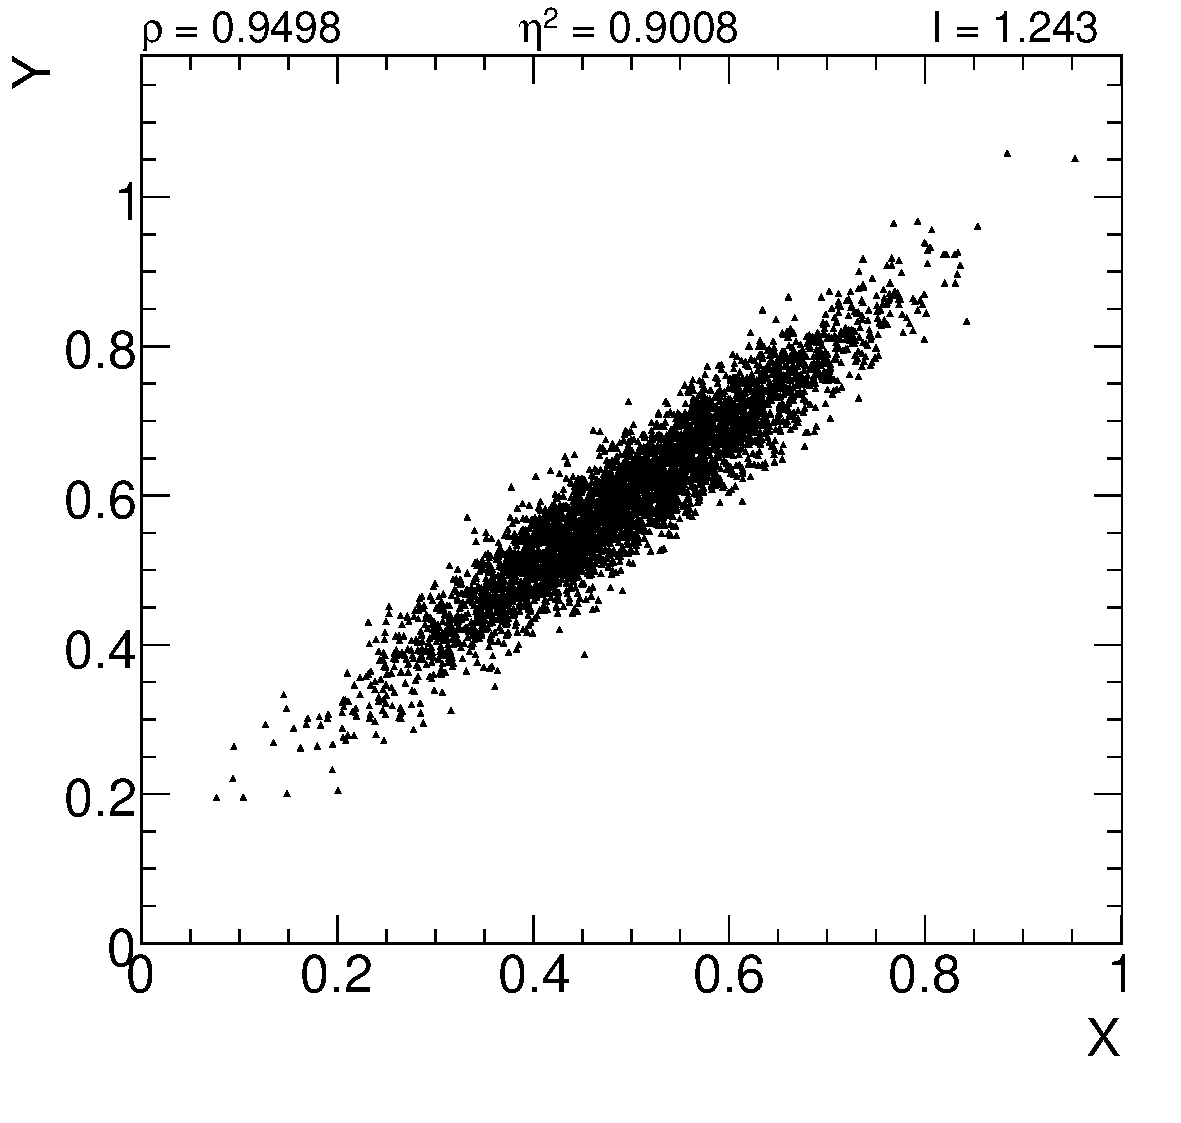
\includegraphics[width=6.2cm]{plots/linDep} \hspace{0.3cm}
  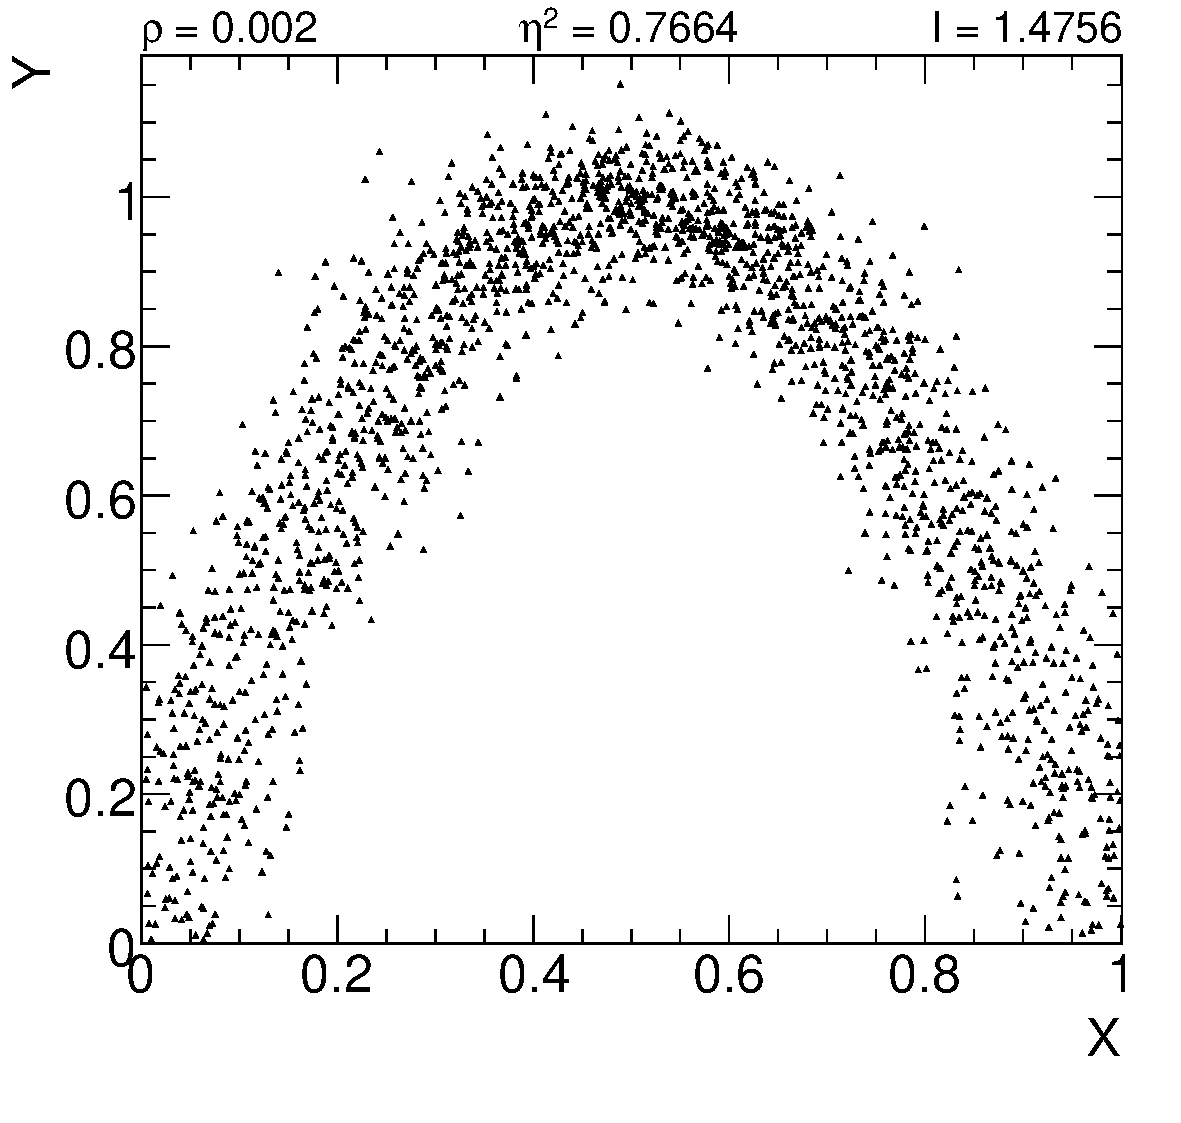
\includegraphics[width=6.2cm]{plots/funcDep} \\\vspace{+0.2cm}
  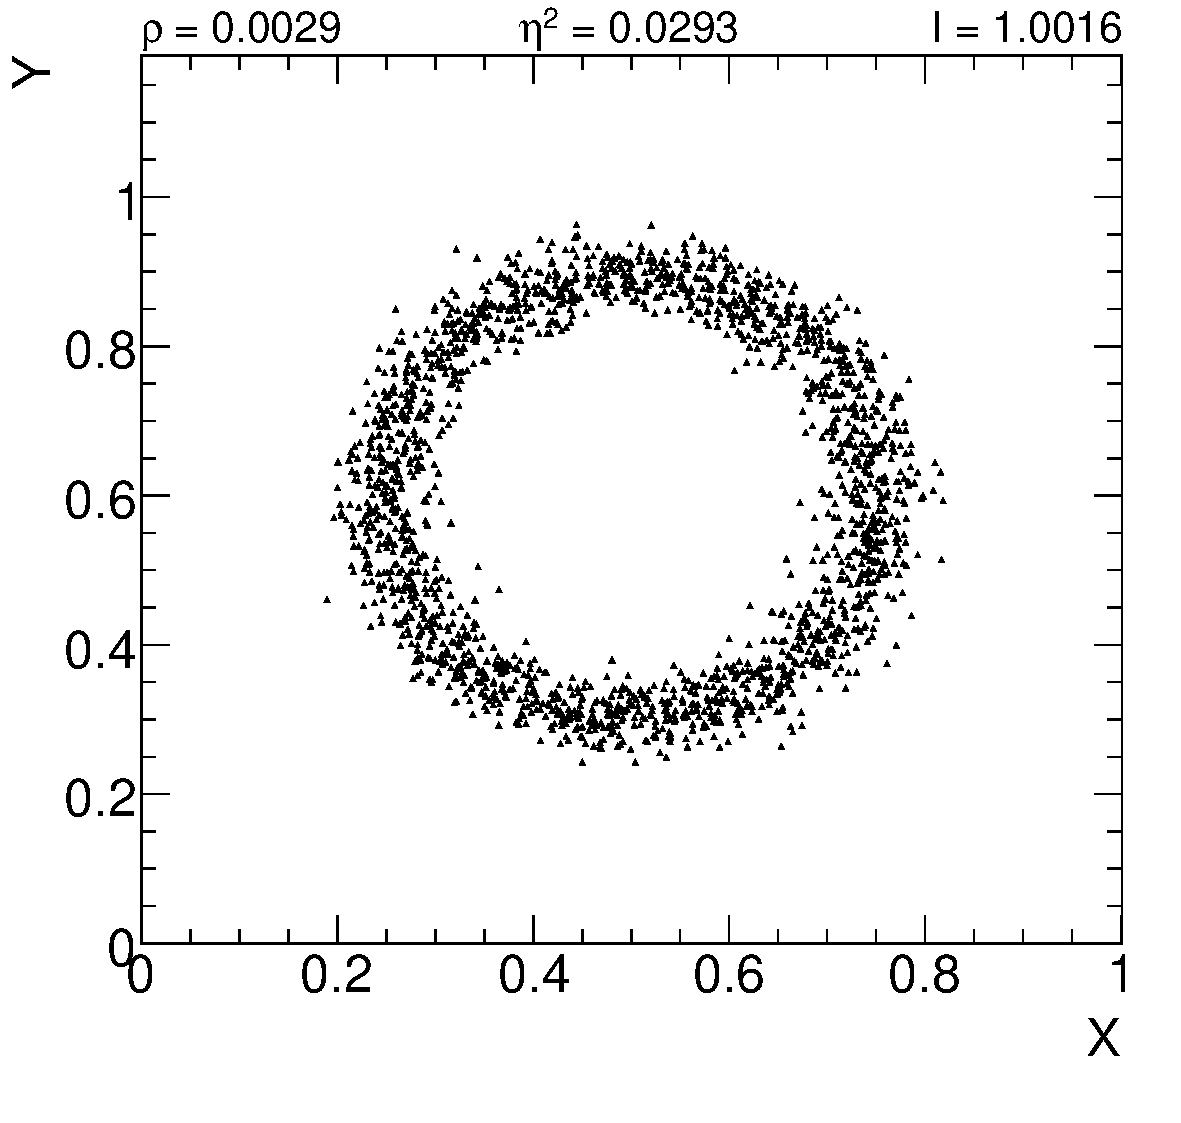
\includegraphics[width=6.2cm]{plots/nonFuncDep} \hspace{0.3cm}
  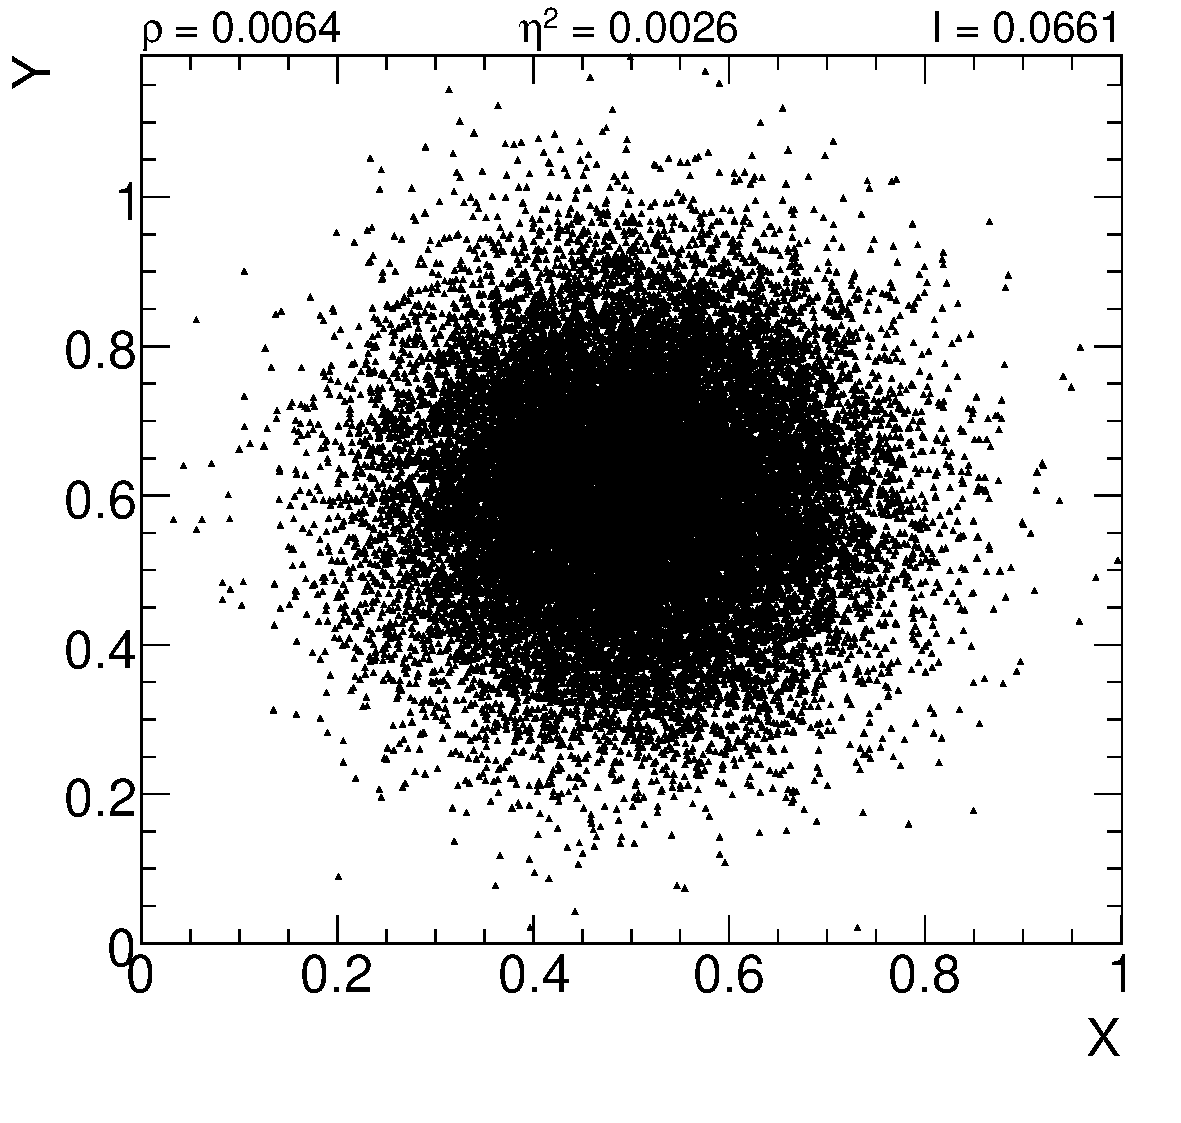
\includegraphics[width=6.2cm]{plots/noDep} 
\end{center}
  \vspace{-0.7cm}
  \caption{Various types of correlations between two random variables
    and their corresponding values for the correlation coefficient
    $\rho$, the correlation ratio $\eta$, and mutual information
    $I$. Linear relationship (upper left), functional relationship
    (upper right), non-functional relationship (lower left), and
    independent variables (lower right).}
  \label{fig:correlationTypes}
\end{figure}
\item {\bf Mutual information} allows to detect any predictable
  relationship between two random variables, be it of functional or
  non-functional form. It is defined by~\cite{citeulike:165404}
      \beq
      \label{eqn:MI}
         I(X,Y) = \sum_{X,Y}P(X,Y) \ln \frac{P(X,Y)}{P(X) P(Y)}\,, 
      \eeq
         where $P(X,Y)$ is the joint probability density function of
         the random variables $X$ and $Y$, and $P(X)$, $P(Y)$ are the
         corresponding marginal probabilities. Mutual information
         originates from information theory and is closely related to
         entropy which is a measure of the uncertainty associated with
         a random variable. It is defined by 
      \beq
      \label{eqn:MIH}
         H(X) = - \sum_{X}P(X) \ln {P(X)}\,, 
         \eeq 
         where $X$ is the
         discrete random variable and $P(X)$ the associated
         probability density function.  The connection between the two
         quantities is given by the following transformation
      \begin{align}
         I(X,Y) &= \sum_{X,Y}P(X,Y) \ln \frac{P(X,Y)}{P(X) P(Y)}\\
           &= \sum_{X,Y}P(X,Y) \ln \frac{P(X|Y)}{P_X(X)}\\
           &= -\sum_{X,Y}P(X,Y) \ln P(X) + \sum_{X,Y}P(X,Y) \ln P(X|Y)\\
           &= -\sum_{X,Y}P(X) \ln P(X) - (-\sum_{X,Y}P(X,Y) \ln P(X|Y) ) \\
           &=H(X) - H(X|Y)\,,	   	
      \end{align}
      where $H(X|Y)$ is the conditional entropy of $X$ given $Y$. Thus
      mutual information is the reduction of the uncertainty in
      variable $X$ due to the knowledge of $Y$. Mutual information is
      symmetric and takes positive absolute values. In the case of two
      completely independent variables $I(X,Y)$ is zero.
      
      For experimental measurements the joint and marginal probability
      density functions are a priori unknown and must be approximated
      by choosing suitable binning procedures such as kernel
      estimation techniques (see, \eg,
      \cite{PhysRevE.52.2318}). Consequently, the values of $I(X,Y)$
      for a given data set will strongly depend on the statistical
      power of the sample and the chosen binning parameters.
      
      For the purpose of ranking variables from data sets of equal
      statistical power and identical binning, however, we assume that
      the evaluation from a simple two-dimensional histogram without
      further smoothing is sufficient.

\end{itemize}
A comparison of the correlation coefficient $\rho$, the correlation
ratio $\eta$, and mutual information $I$ for linearly correlated
two-dimensional Gaussian toy MC simulations is shown in
Table~\ref{tab:compLinToys}.
\begin{table}[t]
\begin{tabularx}{1.0\linewidth}{lXXXXXXXXXXX}
\hline
&&&&&&&&&&&\\[\BD]
$\rho_{\rm PDF}$ & 0.0 & 0.1 & 0.2 & 0.3 & 0.4 & 0.5 & 0.6 & 0.7 & 0.8 & 0.9 & 0.9999\\[\AD]
\hline
&&&&&&&&&&&\\[\BD]
$\rho$ & 0.006& 0.092& 0.191& 0.291& 0.391& 0.492& 0.592& 0.694& 0.795& 0.898& 1.0\\
$\eta^2$& 0.004& 0.012& 0.041& 0.089& 0.156& 0.245& 0.354& 0.484& 0.634& 0.806& 1.0\\
$I$ & 0.093& 0.099& 0.112& 0.139& 0.171& 0.222& 0.295& 0.398& 0.56& 0.861& 3.071\\[\AD]
\hline
\end{tabularx}
\caption{Comparison of the correlation coefficient $\rho$, correlation ratio $\eta$, and 
         mutual information $I$ for two-dimensional Gaussian toy Monte-Carlo distributions 
         with linear correlations as indicated ($20000~{\rm data~points}/100\times100~{\rm bins}$ .}
\label{tab:compLinToys}
\end{table}


\subsubsection{Overtraining\index{Overtraining}}
\label{sec:usingtmva:overtraining}

Overtraining occurs when a machine learning problem has too few
degrees of freedom, because too many model parameters of an algorithm
were adjusted to too few data points. The sensitivity to overtraining
therefore depends on the MVA method.  For example, a Fisher (or {\em
  linear}) discriminant can hardly ever be overtrained, whereas,
without the appropriate counter measures, boosted decision trees
usually suffer from at least partial overtraining, owing to their
large number of nodes.  Overtraining leads to a seeming increase in
the classification or regression performance over the objectively
achievable one, if measured on the training sample, and to an
effective performance decrease when measured with an independent test
sample. A convenient way to detect overtraining and to measure its
impact is therefore to compare the performance results between
training and test samples. Such a test is performed by TMVA with the
results printed to standard output.

Various method-specific solutions to counteract overtraining
exist. For example, binned likelihood reference distributions are
smoothed before interpolating their shapes, or unbinned kernel density
estimators smear each training event before computing the PDF; neural
networks steadily monitor the convergence of the error estimator
between training and test samples\footnote {
   \label{ftn:training}
   Proper training and validation requires three statistically
   independent data sets: one for the parameter optimisation, another
   one for the overtraining detection, and the last one for the
   performance validation. In TMVA, the last two samples have been
   merged to increase statistics. The (usually insignificant) bias
   introduced by this on the evaluation results does not affect the
   analysis as far as classification cut efficiencies or the
   regression resolution are independently validated with data.  }
suspending the training when the test sample has passed its minimum;
the number of nodes in boosted decision trees can be reduced by
removing insignificant ones (``tree pruning''), etc.

\subsubsection{Other representations of MVA outputs for classification: probabilities and probability integral transformation ({\em Rarity})}
\label{sec:otherRepresentations}

In addition to the MVA response value \yMVA of a classifier, which is
typically used to place a cut for the classification of an event as
either signal or background, or which could be used in a subsequent
likelihood fit, TMVA also provides the classifier's signal and
background PDFs, $\yPDFSB$. The PDFs can be used to derive
classification probabilities for individual events, or to compute any
kind of transformation of which the {\em Probability integral transformation} (Rarity) transformation is
implemented in TMVA.
\begin{itemize}

\item {\bf Classification probability}:\index{Classification
  probability} The techniques used to estimate the shapes of the PDFs
  are those developed for the likelihood classifier (see
  Sec.~\ref{sec:likelihood:description} for details) and can be
  customised individually for each method (the control options are
  given in Sec.~\ref{sec:tmvaClassifiers}).  The probability for event
  $i$ to be of signal type is given by\index{Signal probability}, \beq
      \label{eq:proba}
         \proba(i) = \frac{\fS \cdot\yPDFS(i)}{\fS\cdot \yPDFS(i) + (1
           - \fS)\cdot\yPDFB(i)}\,, \eeq where $\fS=\NS/(\NS+\NB)$ is
         the expected signal fraction, and $\NSB$ is the expected
         number of signal (background) events (default is
         $\fS=0.5$).\footnote { The $\proba$ distributions may exhibit
           a somewhat peculiar structure with frequent narrow
           peaks. They are generated by regions of classifier output
           values in which $\yPDFS\propto\yPDFB$ for which $\proba$
           becomes a constant.  }

\item {\bf Probability Integral Transformation}:\index{Rarity} 
      The Probability integral transformation $\Rarity(y)$ of a classifier $y$ is given by the integral~\cite{Rarity}
      \beq
      \label{eq:rarity}
          \Rarity(y) = \intl_{-\infty}^{y}\yPDFB(y^\prime)\,d
          y^\prime~, \eeq which is defined such that $\Rarity(y_B)$
          for background events is uniformly distributed between 0 and
          1, while signal events cluster towards 1. The signal
          distributions can thus be directly compared among the
          various classifiers.  The stronger the peak towards 1, the
          better is the discrimination. Another useful aspect of the
          probability integral transformation is the possibility to directly visualise deviations
          of a test background (which could be physics data) from the
          training sample, by exhibition of non-uniformity.
      
      The probability integral transformation distributions of the Likelihood and Fisher classifiers for the example 
      used in Sec.~\ref{sec:quickstart}
      are plotted in Fig.~\ref{fig:usingtmva:rarity}. Since Fisher performs better
      (\cf\  Fig.~\ref{fig:usingtmva:rejBvsS} on page~\pageref{fig:usingtmva:rejBvsS}),
      its signal distribution is stronger peaked towards 1. By construction, the 
      background distributions are uniform within statistical fluctuations.

\end{itemize}
The probability and probability integral transformation distributions can be plotted with dedicated macros, 
invoked through corresponding GUI buttons.
\begin{figure}[t]
\begin{center}
  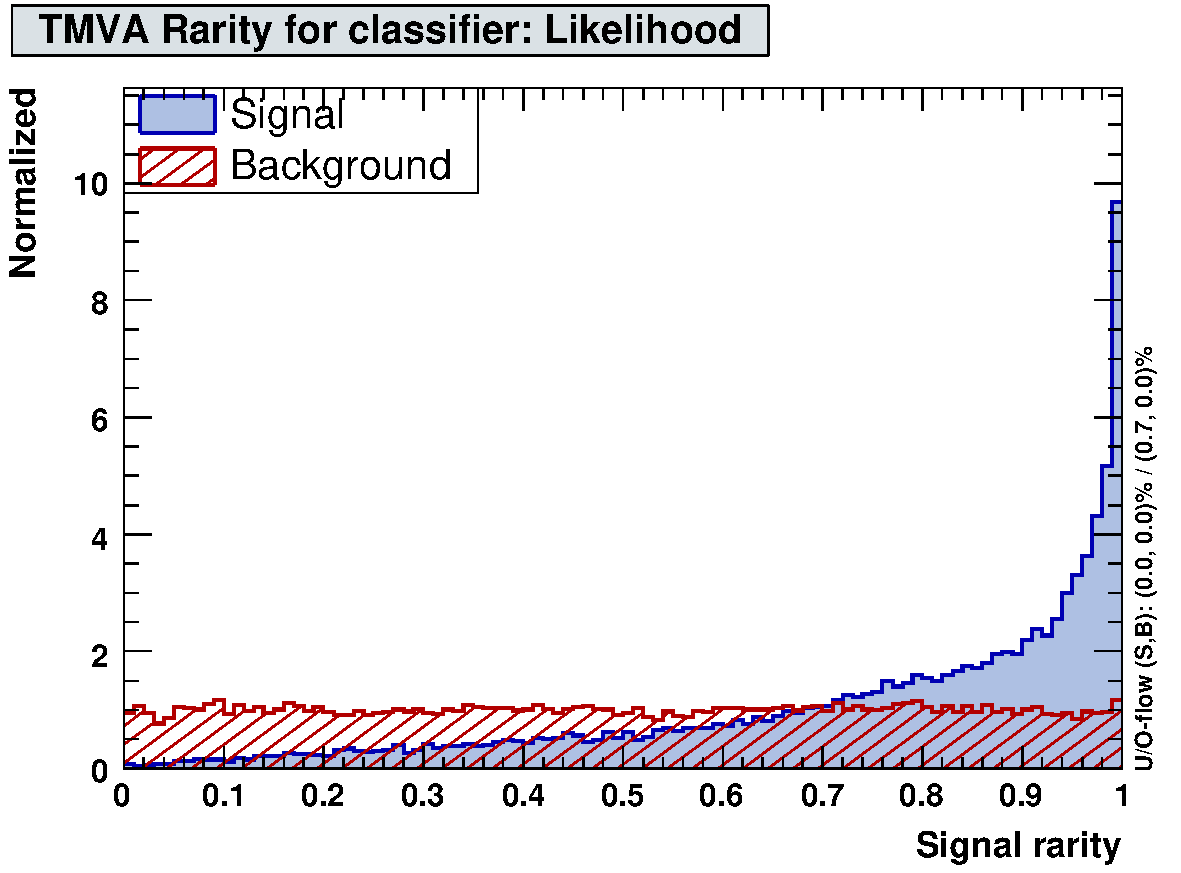
\includegraphics[width=0.50\textwidth]{plots/Rarity-Likelihood}
  \hspace{-0.3cm}
  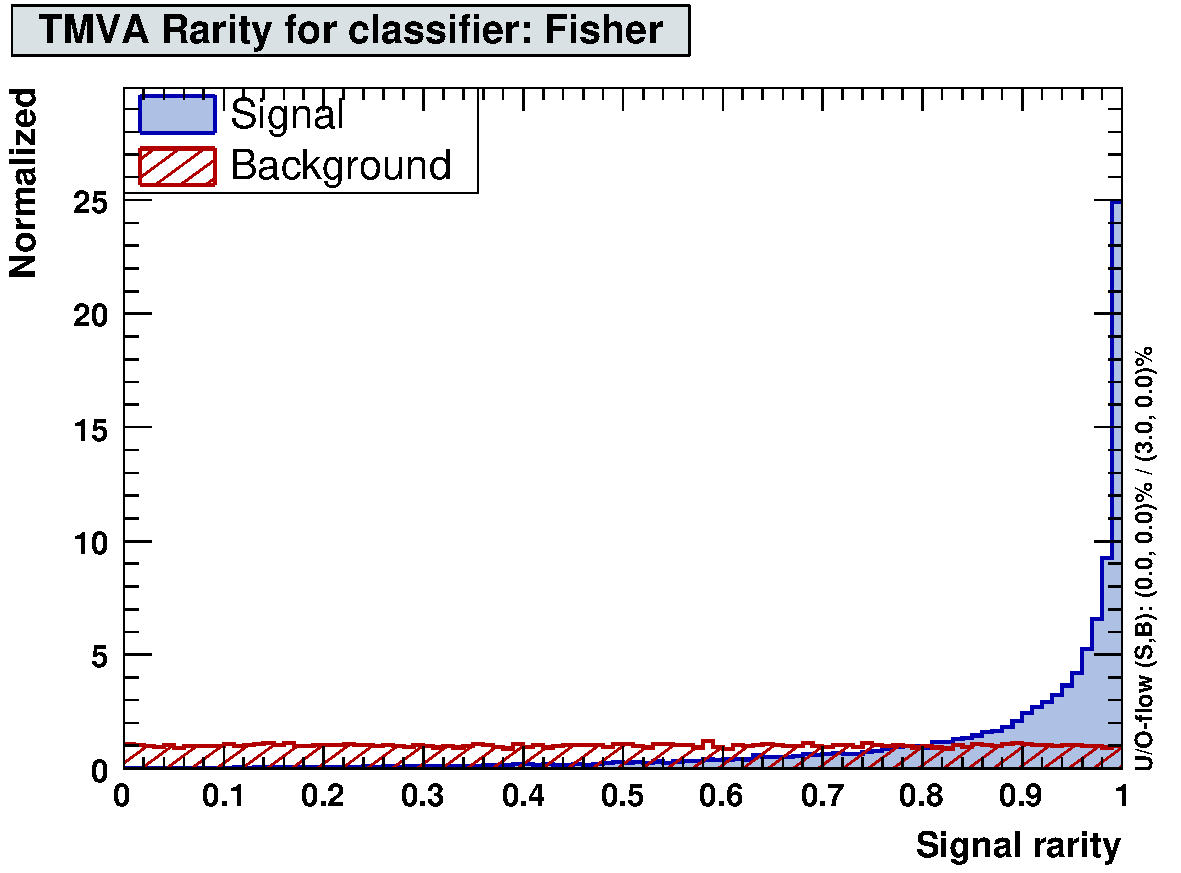
\includegraphics[width=0.50\textwidth]{plots/Rarity-Fisher}
\end{center}
\vspace{-0.5cm}
\caption[.]{Example plots for classifier probability integral transformation distributions for signal and 
            background events from the academic test sample. Shown are
            likelihood (left) and Fisher (right).}
\label{fig:usingtmva:rarity}
\end{figure}

\subsection{ROOT macros to plot training, testing and evaluation 
            results\index{ROOT!macros}}
\label{sec:rootmacros}

TMVA provides simple GUIs (\code{TMVAGui.C} and
\code{TMVARegGui.C}\index{Graphical user interface (GUI)}, see
Fig.~\ref{fig:tmvagui}), which interface ROOT macros that visualise
the various steps of the training analysis. The macros are
respectively located in \code{TMVA/macros/} (Sourceforge.net
distribution) and {\tt \$}\code{ROOTSYS/tmva/test/} (ROOT
distribution), and can also be executed from the command line. They
are described in Tables~\ref{pgr:scripttable1} and
\ref{pgr:scripttable2}. All plots drawn are saved as {\em png} files
(or optionally as {\em eps}, {\em gif} files) in the macro
subdirectory \code{plots} which, if not existing, is created.

The binning and histogram boundaries for some of the histograms
created during the training, testing and evaluation phases are
controlled via the global singleton class \code{TMVA::Config}. They
can be modified as follows:
\begin{codeexample}
\begin{tmvacode}
// Modify settings for the variable plotting
(TMVA::gConfig().GetVariablePlotting()).fTimesRMS = 8.0;
(TMVA::gConfig().GetVariablePlotting()).fNbins1D  = 60.0;
(TMVA::gConfig().GetVariablePlotting()).fNbins2D  = 300.0;

// Modify the binning in the ROC curve (for classification only)
(TMVA::gConfig().GetVariablePlotting()).fNbinsXOfROCCurve = 100;

// For file name settings, modify the struct TMVA::Config::IONames
(TMVA::gConfig().GetIONames()).fWeightFileDir = "myWeightFileDir";
\end{tmvacode}
\caption[.]{\codeexampleCaptionSize Modifying global parameter
  settings for the plotting of the discriminating input variables. The
  values given are the TMVA defaults. Consult the class files
  \href{http://tmva.svn.sourceforge.net/viewvc/tmva/trunk/TMVA/src/Config.h?view=markup}{Config.h}
  and
  \href{http://tmva.svn.sourceforge.net/viewvc/tmva/trunk/TMVA/src/Config.cxx?view=markup}{Config.cxx}
  for all available global configuration variables and their default
  settings, respectively.  Note that the additional parentheses are
  mandatory when used in CINT.}
\label{ce:gconfig}
\end{codeexample}
\begin{table}[p]
\begin{programtable}
variables.C             & Plots the signal and background MVA input variables (training sample).
                          The second argument sets the directory, which determines the 
                          preprocessing type (\code{InputVariables_Id} for default identity 
                          transformation, \cf\  Sec.~\ref{sec:variableTransform}). The third
                          argument is a title, and the fourth argument is a flag whether or not 
                          the input variables served a regression analysis. \\
correlationscatter.C    & Plots superimposed scatters and profiles for all pairs of input 
                          variables used during the training phase (separate plots for 
                          signal and background in case of classification). The arguments
                          are as above.  \\ 
correlations.C          & Plots the linear correlation matrices for the input variables in the 
                          training sample (distinguishing signal and background for classification). \\
mvas.C                  & Plots the classifier response distributions of the test sample for 
                          signal and background. The second argument (\code{HistType=0,1,2,3}) allows 
                          to also plot the probability (1) and probability integral transformation (2) distributions of 
                          the classifiers, as well as a comparison of the output distributions 
                          between test and training samples. 
                          Plotting of probability and probability integral transformation requires 
                          the \code{CreateMVAPdfs} option for the classifier to be set to true. \\
mvaeffs.C               & Signal and background efficiencies, obtained from cutting
                          on the classifier outputs, versus the cut value. Also shown are 
                          the signal purity and the signal efficiency times signal purity
                          corresponding to the expected number of signal and background 
                          events before cutting (numbers given by user). The optimal cuts 
                          according to the best significance are printed on standard output. \\
efficiencies.C          & Background rejection (second argument \code{type=2}, default),
                          or background efficiency (\code{type=1}), versus signal efficiency 
                          for the classifiers (test sample). The efficiencies are
                          obtained by cutting on the classifier outputs. This is traditionally 
                          the best plot to assess the overall discrimination performance (ROC curve).\\   
paracoor.C              & Draws diagrams of ``Parallel coordinates''~\cite{parallelcoor} 
                          for signal and background,
                          used to visualise the correlations among the input variables, 
                          but also between the MVA output and input variables (indicating
                          the importance of the variables).                           
\end{programtable}
\caption[.]{\programCaptionSize ROOT macros for the representation of the 
         TMVA input variables and {\bf classification results}. All macros take as first 
         argument the name of the ROOT file containing the histograms (default is 
         \code{TMVA.root}). They are conveniently called via the \code{TMVAGui.C} GUI
         (the first three macros are also called from the regression GUI \code{TMVARegGui.C}).      
         Macros for the representation of regression results are given in Table~\ref{pgr:scripttable_reg}.    
         Plotting macros for MVA method specific information are listed in 
         Table~\ref{pgr:scripttable2}. 
         \index{ROOT!macros}}
\label{pgr:scripttable1}
\end{table}
\begin{table}[h!]
\begin{programtable}
deviations.C              & Plots the linear deviation between regression target value and MVA 
                            response or input variables for test and training samples. \\
regression\_averagedevs.C & Draws the average deviation between the MVA output and the 
                            regression target value for all trained methods. 
\end{programtable}
\caption[.]{\programCaptionSize ROOT macros for the representation of the 
         TMVA {\bf regression results}. All macros take as first argument the name of 
         the ROOT file containing the histograms (default is \code{TMVA.root}). They 
         are conveniently called from the \code{TMVARegGui.C} GUI. 
         \index{ROOT!macros}}
\label{pgr:scripttable_reg}
\end{table}
\begin{table}[t]
\begin{programtable}
likelihoodrefs.C  	   & Plots the reference PDFs of all 
                          input variables for the projective likelihood method and compares it 
                          to original distributions obtained from the training sample.  \\
network.C 	            & Draws the TMVA-MLP architecture including weights after training (does 
                          not work for the other ANNs).                     \\
annconvergencetest.C    & Plots the MLP error-function convergence versus the training epoch 
                          for training and test events (does not work for the other ANNs). \\
BDT.C(i)                & Draws the \code{i}th decision tree of the trained forest (default is 
                          \code{i=1}). The second argument is the weight file that contains 
                          the full architecture of the forest (default is
                          \code{weights/TMVAClassification_BDT.weights.xml}). \\
BDTControlPlots.C       & Plots distributions of boost weights throughout forest, 
                          boost weights versus decision tree, error fraction, number of nodes
                          before and after pruning and the coefficient $\alpha$.\\
mvarefs.C               & Plots the PDFs used to compute the probability response for a classifier, 
                          and compares it to the original distributions. \\
PlotFoams.C             & Draws the signal and background foams created by the method 
                          PDE-Foam.\\
rulevis.C               & Plots the relative importance of rules and linear terms.
                          The 1D plots show the accumulated importance per input variable. 
                          The 2D scatter plots show the same but correlated between the 
                          input variables. These plots help to identify regions in the 
                          parameter space that are important for the model.
\end{programtable}
\caption[.]{\programCaptionSize List of ROOT macros representing results for 
            {\bf specific MVA methods}. The macros require that these methods have been 
            included in the training. All macros take as first argument the name of the 
            ROOT file containing the histograms (default is \code{TMVA.root}).}
\label{pgr:scripttable2}
\end{table}

\subsection{The TMVA Reader\index{Reader}}
\label{sec:usingtmva:reader}

After training and evaluation, the most performing MVA methods are chosen and 
used to classify events in data samples with unknown signal and background composition,
or to predict values of a regression target. An example of how this {\em application phase} 
is carried out is given in \code{TMVA/macros/TMVAClassificationApplication.C} and
\code{TMVA/macros/TMVARegressionApplication.C} (Sourceforge.net), or 
{\tt \$}\code{ROOTSYS/tmva/test/TMVAClassificationApplication.C} and
{\tt \$}\code{ROOTSYS/tmva/test/TMVARegressionApplication.C} (ROOT).

Analogously to the Factory, the communication between the user application and 
the MVA methods is interfaced by the TMVA {\em Reader}, which is created by 
the user:
\begin{codeexample}
\begin{tmvacode}
TMVA::Reader* reader = new TMVA::Reader( "<options>" );
\end{tmvacode}
\caption[.]{\codeexampleCaptionSize Instantiating a Reader class object. The only
            options are the booleans: \code{V} for verbose, \code{Color} for coloured output, 
            and \code{Silent} to suppress all output.}
\end{codeexample}

\subsubsection{Specifying input variables\index{Reader!specifying input variables}}

The user registers the names of the input variables with the Reader. They are
required to be the same (and in the same order) as the names used for training 
(this requirement is not actually mandatory, but enforced to ensure the consistency 
between training and application). Together with the name is given the address of a 
local variable, which carries the updated input values during the event loop.
\begin{codeexample}
\begin{tmvacode}
Int_t   localDescreteVar;
Float_t localFloatingVar, locaSum, localVar3;

reader->AddVariable( "<YourDescreteVar>",                 &localDescreteVar );
reader->AddVariable( "log(<YourFloatingVar>)",            &localFloatingVar );
reader->AddVariable( "SumLabel := <YourVar1>+<YourVar2>", &locaSum          );
reader->AddVariable( "<YourVar3>",                        &localVar3        );
\end{tmvacode}
\caption[.]{\codeexampleCaptionSize Declaration of the variables and references 
            used as input to the methods (\cf Code Example~\ref{ce:addvariable}). 
            The order and naming of the variables
            must be consistent with the ones used for the training. The local 
            variables are updated during the event loop, and through the references
            their values are known to the MVA methods. The variable type must be either
            \code{float} or \code{int} (\code{double} is not supported). }
\end{codeexample}

\subsubsection{Booking MVA methods\index{Reader!booking MVA methods}}

The selected MVA methods are booked with the Reader using the weight files from the 
preceding training job:\index{Weight files!XML format}
\begin{codeexample}
\begin{tmvacode}
reader->BookMVA( "<YourMethodName>", "<path/JobName_MethodName.weights.xml>" );
\end{tmvacode}
\caption[.]{\codeexampleCaptionSize Booking a multivariate method. The first
            argument is a user defined name to distinguish between  
            methods (it does not need to be the same name as for training, 
            although this could be a useful choice). The true type of the 
            method and its full configuration are read from the weight file
            specified in the second argument. The default structure of the 
            weight file names is: \code{path/<JobName>_<MethodName>.weights.xml}.
}
\end{codeexample}

\subsubsection{Requesting the MVA response\index{Reader!requesting the MVA response}}

Within the event loop, the response value of a classifier, and -- if available -- 
its error, for a given set of input variables computed by the user, are obtained 
with the commands:
\begin{codeexample}
\begin{tmvacode}
localDescreteVar  = treeDescreteVar;       // reference could be implicit
localFloatingVar  = log(treeFloatingVar);
locaSum           = treeVar1 + treeVar2;
localVar3         = treeVar3;              // reference could be implicit

// Classifier response
Double_t mvaValue = reader->EvaluateMVA( "<YourMethodName>" );

// Error on classifier response - must be called after "EvaluateMVA"
// (not available for all methods, returns -1 in that case)
Double_t mvaErr   = reader->GetMVAError();
\end{tmvacode}
\caption[.]{\codeexampleCaptionSize Updating the local variables for an event, 
            and obtaining the corresponding classifier output and error 
            (if available -- see text). }
\end{codeexample}
The output of a classifier may then be used for example to put a cut that increases the 
signal purity of the sample (the achievable purities can be read off the evaluation
results obtained during the test phase), or it could enter a subsequent 
maximum-likelihood fit, or similar. The error reflects the uncertainty, which 
may be statistical, in the output value as obtained from the training information. 

For regression, multi-target response is already supported in TMVA, so that the 
retrieval command reads:
\begin{codeexample}
\begin{tmvacode}
// Regression response for one target
Double_t regValue = (reader->EvaluateRegression( "<YourMethodName>" ))[0];
\end{tmvacode}
\caption[.]{\codeexampleCaptionSize Obtaining the regression output (after 
            updating the local variables for an event -- see above). For mult-target 
            regression, the corresponding vector entries are filled.}
\end{codeexample}
The output of a regression method could be directly used for example as energy estimate 
for a calorimeter cluster as a function of the cell energies. 

The rectangular cut classifier is special since it returns a binary answer for a given 
set of input variables and cuts. The user must specify the desired signal efficiency
to define the working point according to which the Reader will choose the cuts:
\begin{codeexample}
\begin{tmvacode}
Bool_t passed = reader->EvaluateMVA( "Cuts", signalEfficiency );
\end{tmvacode}
\caption[.]{\codeexampleCaptionSize For the cut classifier, the second parameter 
            gives the desired signal efficiency according to which the cuts 
            are chosen. The return value is 1 for passed and 0 for retained. 
            See Footnote~\ref{ftn:cutcomp} on page~\pageref{ftn:cutcomp} for 
            information on how to determine the optimal working point for 
            known signal and background abundance.}
\end{codeexample}

Instead of the classifier response values, one may also retrieve the ratio~(\ref{eq:proba})
from the Reader, which, if properly normalised to the expected signal fraction 
in the sample, corresponds to a probability. The corresponding command
reads:\index{Reader!requesting the signal probability of a classifier}
\begin{codeexample}
\begin{tmvacode}
Double_t pSig = reader->GetProba( "<YourClassifierName>", sigFrac );
\end{tmvacode}
\caption[.]{\codeexampleCaptionSize Requesting the event's signal probability from a 
            classifier. The signal fraction is the parameter $\fS$ in Eq.~(\ref{eq:proba}).}
\end{codeexample}
Similarly, the probability integral transformation ({\em Rarity})~(\ref{eq:rarity}) of a classifier is retrieved by the 
command\index{Reader!requesting the Rarity of a classifier}
\begin{codeexample}
\begin{tmvacode}
Double_t rarity = reader->GetRarity( "<YourClassifierName>" );
\end{tmvacode}
\caption[.]{\codeexampleCaptionSize Requesting the event's probability integral transformation distribution from a 
            classifier. }
\end{codeexample}

\subsection{An alternative to the Reader: standalone C++ response classes
           \index{Standalone C++ response classes}}
\label{sec:usingtmva:standaloneClasses}

\begin{codeexample}[tb]
\begin{tmvacode}
// load the generated response class into macro and compile it (ROOT)
// or include it into any C++ executable
gROOT->LoadMacro( "TMVAClassification_Fisher.class.C++" ); // usage in ROOT 

// define the names of the input variables (same as for training)
std::vector<std::string> inputVars;
inputVars.push_back( "<YourVar1>" );
inputVars.push_back( "log(<YourVar2>)" );
inputVars.push_back( "<YourVar3>+<YourVar4>" );

// create a class object for the Fisher response
IClassifierReader* fisherResponse = new ReadFisher( inputVars );

// the user's event loop ...
std::vector<double> inputVec( 3 );
for (...) {
   // compute the input variables for the event
   inputVec[0] = treeVar1;
   inputVec[1] = TMath::Log(treeVar2);
   inputVec[2] = treeVar3 + treeVar4;

   // get the Fisher response
   double fiOut = fisherResponse->GetMvaValue( inputVec );
   // ... use fiOut
}
\end{tmvacode}
\caption[.]{\codeexampleCaptionSize
            Using a standalone C++ class for the classifier
            response in an application (here of the Fisher discriminant). See also the 
            example code in \code{TMVA/macros/ClassApplication.C} (Sourceforge.net).}
\label{ce:standaloneClasses}
\end{codeexample}
To simplify the portability of the trained MVA response to any application the TMVA 
methods generate after the training lightweight standalone C++ response classes 
including in the source code the content of the weight files.\footnote
{
   At present, the class making functionality has been implemented for 
   all MVA methods with the exception of cut optimisation, PDE-RS, PDE-Foam and k-NN. While 
   for the former classifier the cuts can be easily implemented into the user application, 
   and do not require an extra class, the implementation of a response class for
   PDE-RS or k-NN requires a copy of the entire analysis code, which we have not 
   attempted so far. We also point out that the use of the standalone C++ class
   for BDT is not practical due to the colossal size of the generated code. 
} 
These classes do not depend on ROOT, neither on any other non-standard library.
The names of the classes are constructed out of \code{Read+"MethodName"}, and
they inherit from the interface class \code{IClassifierReader}, which is written 
into the same C++ file. These standalone classes are {\em presently only available 
for classification}.

An example application (ROOT script here, not representative
for a C++ standalone application) for a Fisher classifier is given in 
Code-Example~\ref{ce:standaloneClasses}. The example is also available in the macro
\code{TMVA/macros/ClassApplication.C} (Sourceforge.net). These classes are C++ 
representations of the information stored in the weight files. Any change in the 
training parameters will generate a new class, which must be updated in the 
corresponding application.\footnote
{
   We are aware that requiring recompilation constitutes a significant shortcoming.
   we consider to upgrade these classes to reading the XML weight files, which
   entails significant complications if the independence of any external 
   library shall be conserved. 
} 

For a given test event, the MVA response returned by the standalone class 
is identical to the one returned by the Reader. Nevertheless, {\em we emphasise that 
the recommended approach to apply the training results is via the Reader}. 
\clearpage
